\chapter{Evaluation}\label{evaluation}

\section{Evaluation Framework and Scope}\label{evaluation-framework-and-scope}

The role of this chapter is to evaluate Intelli-Trading Fours not as a
finished autonomous musical performer but as a technical interaction
system. As previously established, the implemented contribution is a
closed-loop prototype for turn-based human-AI rhythmic exchange,
encompassing: input capture, symbolic representation, rhythmic analysis,
response planning, playback and return to a ready state for repeated
interaction. The purpose of this evaluation is therefore not to assess
artistic quality in isolation, but to determine whether the system
behaves as intended according to the design decisions established in
Chapter 3.

Accordingly, the chapter adopts an evidence-driven, architecture-level
evaluation framework where the system is assessed through a combination
of:

\begin{itemize}
\item
  subsystem tests
\item
  batch diagnostic outputs
\item
  runtime observability tools
\item
  structural analysis metrics
\end{itemize}

Subsystem correctness is validated through unit and integration testing
at each state phase. Higher-level behaviour is examined using
large-scale batch output data (e.g. statistical distributions,
structural divergence measures), curated case studies and controlled
input-variation experiments. Runtime debug interfaces also provide
direct observability into internal system states, facilitating
interpretability past relying solely on output inspection.

To operationalise this framework, evaluation is organised around the
following core questions:

\begin{itemize}
\item
  Does the system demonstrate stable closed-loop interaction across
  repeated turns?
\item
  Are response planning decisions interpretable and internally
  consistent?
\item
  Do different response types produce structurally distinct rhythmic
  outputs?
\item
  Does the system exhibit reactivity, such that variations in input lead
  to meaningful variations in response?
\item
  Does the system operate within real-time constraints, particularly in
  post-capture latency?
\item
  To what extent is planner intent preserved in the generated output and
  where does this break down?
\end{itemize}

\begin{longtable}[]{@{}
  >{\raggedright\arraybackslash}p{(\linewidth - 8\tabcolsep) * \real{0.2738}}
  >{\raggedright\arraybackslash}p{(\linewidth - 8\tabcolsep) * \real{0.0780}}
  >{\raggedright\arraybackslash}p{(\linewidth - 8\tabcolsep) * \real{0.2487}}
  >{\raggedright\arraybackslash}p{(\linewidth - 8\tabcolsep) * \real{0.2050}}
  >{\raggedright\arraybackslash}p{(\linewidth - 8\tabcolsep) * \real{0.1944}}@{}}
\caption{Evaluation questions and evidence sources}\label{tab:evaluation-framework}\\
\toprule\noalign{}
\begin{minipage}[b]{\linewidth}\centering
\textbf{Evaluation Question}
\end{minipage} & \begin{minipage}[b]{\linewidth}\centering
\textbf{Claim Type}
\end{minipage} & \begin{minipage}[b]{\linewidth}\centering
\textbf{Evidence Source(s)}
\end{minipage} & \begin{minipage}[b]{\linewidth}\centering
\textbf{Method of Analysis}
\end{minipage} & \begin{minipage}[b]{\linewidth}\centering
\textbf{Output (Figure/Table)}
\end{minipage} \\
\begin{minipage}[b]{\linewidth}\raggedright
Does the system demonstrate stable closed-loop interaction?
\end{minipage} & \begin{minipage}[b]{\linewidth}\raggedright
Strong
\end{minipage} & \begin{minipage}[b]{\linewidth}\raggedright
Integration tests, TurnLoopController execution, runtime logs
\end{minipage} & \begin{minipage}[b]{\linewidth}\raggedright
End-to-end execution validation, phase consistency checks
\end{minipage} & \begin{minipage}[b]{\linewidth}\raggedright
System flow diagram, execution trace (Figure~\ref{fig:abstracted-turn-loop-state-trace})
\end{minipage} \\
\begin{minipage}[b]{\linewidth}\raggedright
Are planning decisions interpretable and internally consistent?
\end{minipage} & \begin{minipage}[b]{\linewidth}\raggedright
Strong
\end{minipage} & \begin{minipage}[b]{\linewidth}\raggedright
Planner CSV (300 runs), planner debug output
\end{minipage} & \begin{minipage}[b]{\linewidth}\raggedright
Distribution analysis, margin analysis, rule consistency inspection
\end{minipage} & \begin{minipage}[b]{\linewidth}\raggedright
Planner distribution (Figure~\ref{fig:planner-response-type-distribution}), margin plot (Figure~\ref{fig:planner-decision-margin-distribution})
\end{minipage} \\
\begin{minipage}[b]{\linewidth}\raggedright
Do response types produce structurally distinct outputs?
\end{minipage} & \begin{minipage}[b]{\linewidth}\raggedright
Strong
\end{minipage} & \begin{minipage}[b]{\linewidth}\raggedright
Skeleton batch outputs (1800 cases), structural metrics
\end{minipage} & \begin{minipage}[b]{\linewidth}\raggedright
Overlap, divergence, anchor preservation, gap-fill analysis
\end{minipage} & \begin{minipage}[b]{\linewidth}\raggedright
Structural metrics table (Table~\ref{tab:structural-metrics-summary}), divergence plot (Figure~\ref{fig:structural-divergence-distribution})
\end{minipage} \\
\begin{minipage}[b]{\linewidth}\raggedright
Does the system exhibit reactivity to input variation?
\end{minipage} & \begin{minipage}[b]{\linewidth}\raggedright
Partial
\end{minipage} & \begin{minipage}[b]{\linewidth}\raggedright
Variant dataset (input perturbations), planner outputs
\end{minipage} & \begin{minipage}[b]{\linewidth}\raggedright
Sensitivity analysis (response type changes vs input changes)
\end{minipage} & \begin{minipage}[b]{\linewidth}\raggedright
Variant sensitivity table/plot (Figure~\ref{fig:variant-sensitivity})
\end{minipage} \\
\begin{minipage}[b]{\linewidth}\raggedright
Does the system operate within real-time constraints?
\end{minipage} & \begin{minipage}[b]{\linewidth}\raggedright
Partial
\end{minipage} & \begin{minipage}[b]{\linewidth}\raggedright
Timing logs (capture \(\rightarrow\) playback), runtime profiling
\end{minipage} & \begin{minipage}[b]{\linewidth}\raggedright
Latency measurement (post-capture delay, stage timings)
\end{minipage} & \begin{minipage}[b]{\linewidth}\raggedright
Latency plot (TODO: missing latency plot figure source)
\end{minipage} \\
\begin{minipage}[b]{\linewidth}\raggedright
Is planner intent preserved in generated output?
\end{minipage} & \begin{minipage}[b]{\linewidth}\raggedright
Partial
\end{minipage} & \begin{minipage}[b]{\linewidth}\raggedright
Curated cases, plan vs output dataset
\end{minipage} & \begin{minipage}[b]{\linewidth}\raggedright
Structural comparison (density, overlap, pattern alignment)
\end{minipage} & \begin{minipage}[b]{\linewidth}\raggedright
Plan vs output comparison (Figure~\ref{fig:plan-output-density-error}), case table (TODO: missing plan-vs-output case table source)
\end{minipage} \\
\begin{minipage}[b]{\linewidth}\raggedright
Is the system musically plausible as an interaction partner?
\end{minipage} & \begin{minipage}[b]{\linewidth}\raggedright
Partial
\end{minipage} & \begin{minipage}[b]{\linewidth}\raggedright
Curated outputs, qualitative inspection
\end{minipage} & \begin{minipage}[b]{\linewidth}\raggedright
Case-based interpretation (no user study)
\end{minipage} & \begin{minipage}[b]{\linewidth}\raggedright
Annotated case figures (Figure~\ref{fig:planner-decision-trace}; TODO: add annotated case figure if available)
\end{minipage} \\
\begin{minipage}[b]{\linewidth}\raggedright
Does the system support perceptual or user-level evaluation?
\end{minipage} & \begin{minipage}[b]{\linewidth}\raggedright
Deferred
\end{minipage} & \begin{minipage}[b]{\linewidth}\raggedright
-
\end{minipage} & \begin{minipage}[b]{\linewidth}\raggedright
Not evaluated in this work
\end{minipage} & \begin{minipage}[b]{\linewidth}\raggedright
-
\end{minipage} \\
\begin{minipage}[b]{\linewidth}\raggedright
Does the system support long-term adaptation or learning?
\end{minipage} & \begin{minipage}[b]{\linewidth}\raggedright
Deferred
\end{minipage} & \begin{minipage}[b]{\linewidth}\raggedright
-
\end{minipage} & \begin{minipage}[b]{\linewidth}\raggedright
Not implemented
\end{minipage} & \begin{minipage}[b]{\linewidth}\raggedright
-
\end{minipage} \\
\midrule\noalign{}
\endhead
\bottomrule\noalign{}
\endlastfoot
\end{longtable}


Each of these questions corresponds to a specific class of evidence
(tests, batch data, timing logs, or curated cases) supported by figures
and tables derived directly from system outputs. This ensures that
evaluation claims are grounded in measurable behaviour rather than
descriptive assertion.

The scope of evaluation is intentionally constrained. This chapter is
not intended to establish perceptual musical quality, listener
satisfaction, or the effectiveness of the system as a fully realised
co-creative partner. While these aspects broadly relate to interactive
music systems, they are beyond the current scope. Instead, the focus is
on whether the system functions as a coherent, interpretable and
responsive interaction architecture - identifying the extent to which
this goal has been achieved.

This distinction is critical when interpreting results. Structural and
computational evidence can demonstrate that the system is responsive,
internally consistent and capable of differentiated behaviour, but
cannot alone establish artistic success. For this reason, the evaluation
separates strongly evidenced claims (e.g. architectural correctness,
planner interpretability, structural differentiation), partially
evidenced claims (e.g. real-time responsiveness, plan-to-output
fidelity, musical plausibility) and explicitly deferred claims (e.g.
user evaluation, long-term adaptation, fully expressive generation).

By structuring the evaluation in this way, Chapter 5 reinforces
Intelli-Trading Fours not as a completed musical system, but as a
well-instrumented, technically grounded prototype, whose behaviour can
be rigorously analysed, whose scope is outlined and whose design
decisions can be critically assessed within the broader context of
interactive musical systems.

\section{Implementation Validation}\label{implementation-validation}

This section validates the correctness of the Intelli-Trading Fours
system as an integrated, closed-loop interaction architecture. The aim
is to establish that the system executes reliably across its full
interaction cycle.

At a system level, Intelli-Trading Fours is designed as a phase-based
interaction loop, consisting of sequential stages: input capture, turn
segmentation, symbolic compilation, rhythmic analysis, response
planning, response generation, playback and transition back to a ready
state. Validation therefore focuses on confirming that each stage
executes correctly in isolation and that transitions between stages
occur deterministically and without failure.

To support this, a combination of unit testing, integration testing and
runtime validation is employed.

Unit tests verify the correctness of individual subsystems, including
feature extraction, response planning logic and skeleton generation
behaviour providing a baseline guarantee of correctness at the subsystem
level.

Integration testing extends this validation to the full interaction
loop. Controlled input sequences are passed through the system to
confirm that the pipeline executes without interruption, that state
transitions occur in the correct order and that outputs are produced at
the expected stages. Particular attention is given to the
TurnLoopController, which orchestrates the interaction phases, ensuring
that transitions such as Capturing \(\rightarrow\) Compiling \(\rightarrow\) Planning \(\rightarrow\) Playback
occur consistently and without race conditions or dead states.

In addition to formal tests, runtime observability tools are used to
validate behaviour during execution. Debug interfaces provide real-time
visualisation of internal representations, including captured hit
events, quantised PatternTurn structures, extracted features, planner
outputs and generated response patterns. This allows verification not
only that the system produces outputs, but that intermediate
representations remain coherent and interpretable throughout execution.
Such observability is particularly important in interactive systems,
where silent failures or misalignments between stages may not be
immediately apparent from output alone.

The results of this validation indicate that the system reliably
completes the full interaction cycle under controlled conditions. Input
events are successfully captured and segmented into discrete turns,
symbolic representations are constructed consistently, analysis and
planning stages execute deterministically and response playback is
triggered without failure. The system also consistently returns to a
ready state following playback, enabling repeated interaction cycles
without manual reset.

Overall, this section establishes that Intelli-Trading Fours satisfies
its core requirement as a working closed-loop interaction system,
providing a stable foundation for the behavioural and structural
evaluations that follow.

The runtime traces in Figure~\ref{fig:example-system-execution-trace} and Figure~\ref{fig:abstracted-turn-loop-state-trace} show the progression through capture, compilation, response generation and playback phases. Annotations indicate key events derived from runtime logs, demonstrating deterministic execution and successful loop closure.

\begin{figure}[htbp]
\centering
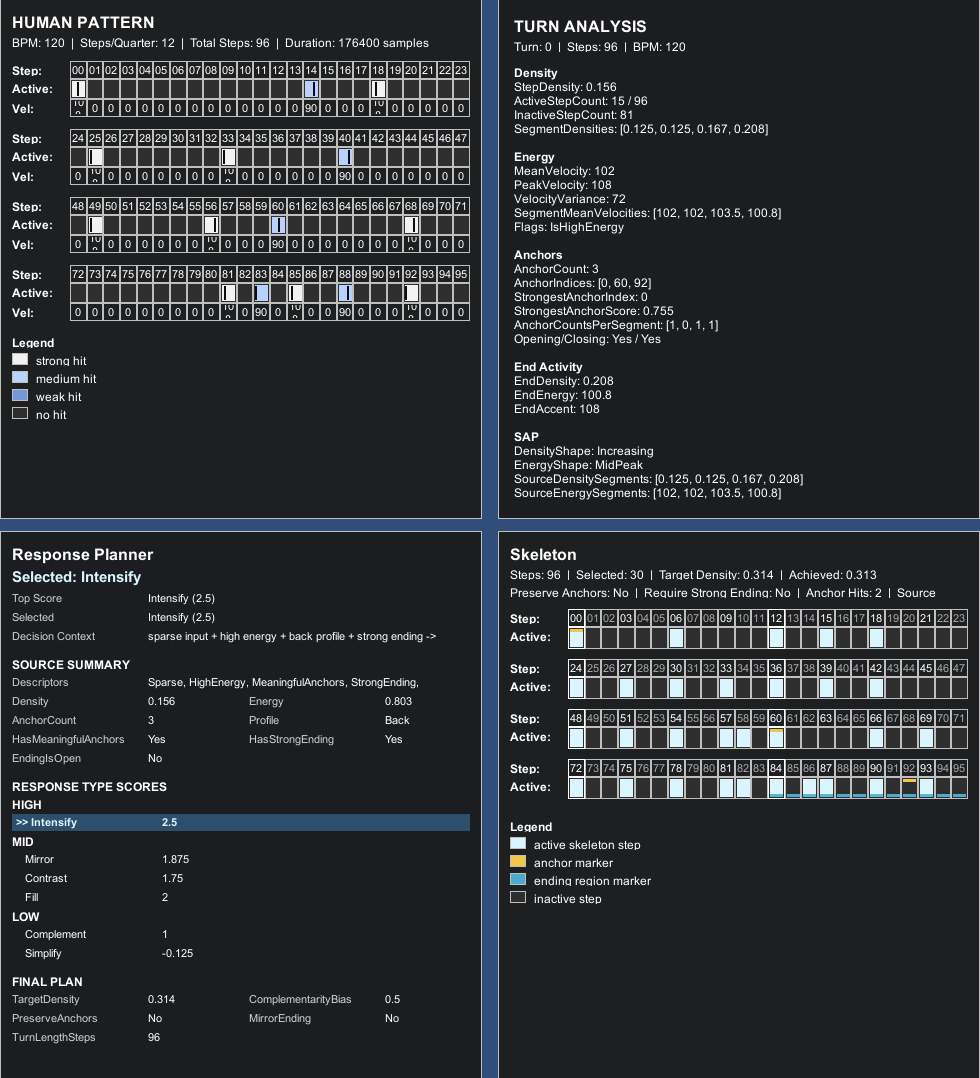
\includegraphics[width=\textwidth]{Figures/5.2 Figs/Figure 5.1 - Example System Execution Trace.png}
\caption{Example system execution trace captured from runtime validation.}
\label{fig:example-system-execution-trace}
\end{figure}

\begin{figure}[htbp]
\centering
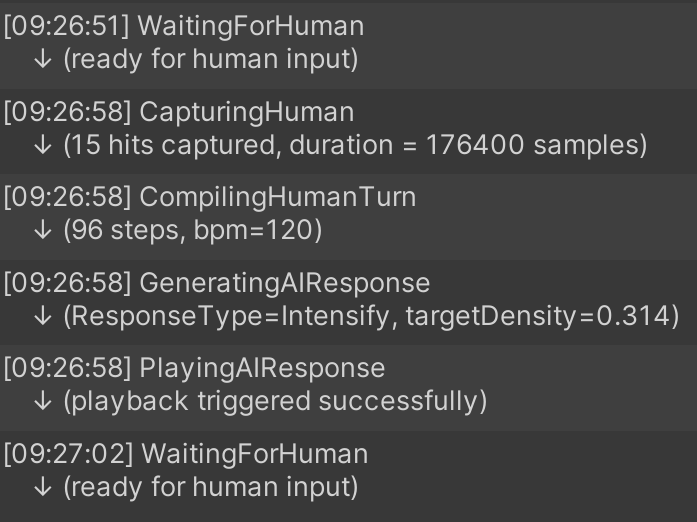
\includegraphics[width=\textwidth]{Figures/5.2 Figs/Figure 5.2 - Abstracted Turn Loop State Trace.png}
\caption{Abstracted state transition trace of the interaction loop.}
\label{fig:abstracted-turn-loop-state-trace}
\end{figure}

\section{Planner Behaviour, Interpretability \& Reactivity}\label{planner-behaviour-interpretability-reactivity}

The response planner forms one of the central decision-making components
of Intelli-Trading Fours, translating analysed rhythmic features into an
explicit response intention. Unlike end-to-end generative systems, the
planner functions as an interpretable intermediate layer, making its
behaviour directly inspectable. This section evaluates the planner in
terms of response diversity, decision confidence, interpretability and
sensitivity to input variation.

\subsection{Distribution of response types}\label{distribution-of-response-types}

A primary requirement of the planner is that it should produce a range
of response types rather than collapsing to a single dominant strategy,
thus exhibiting non-degenerate behaviour.

Figure~\ref{fig:planner-response-type-distribution} shows the distribution of selected response types across 300 analysed cases.

\begin{figure}[htbp]
\centering
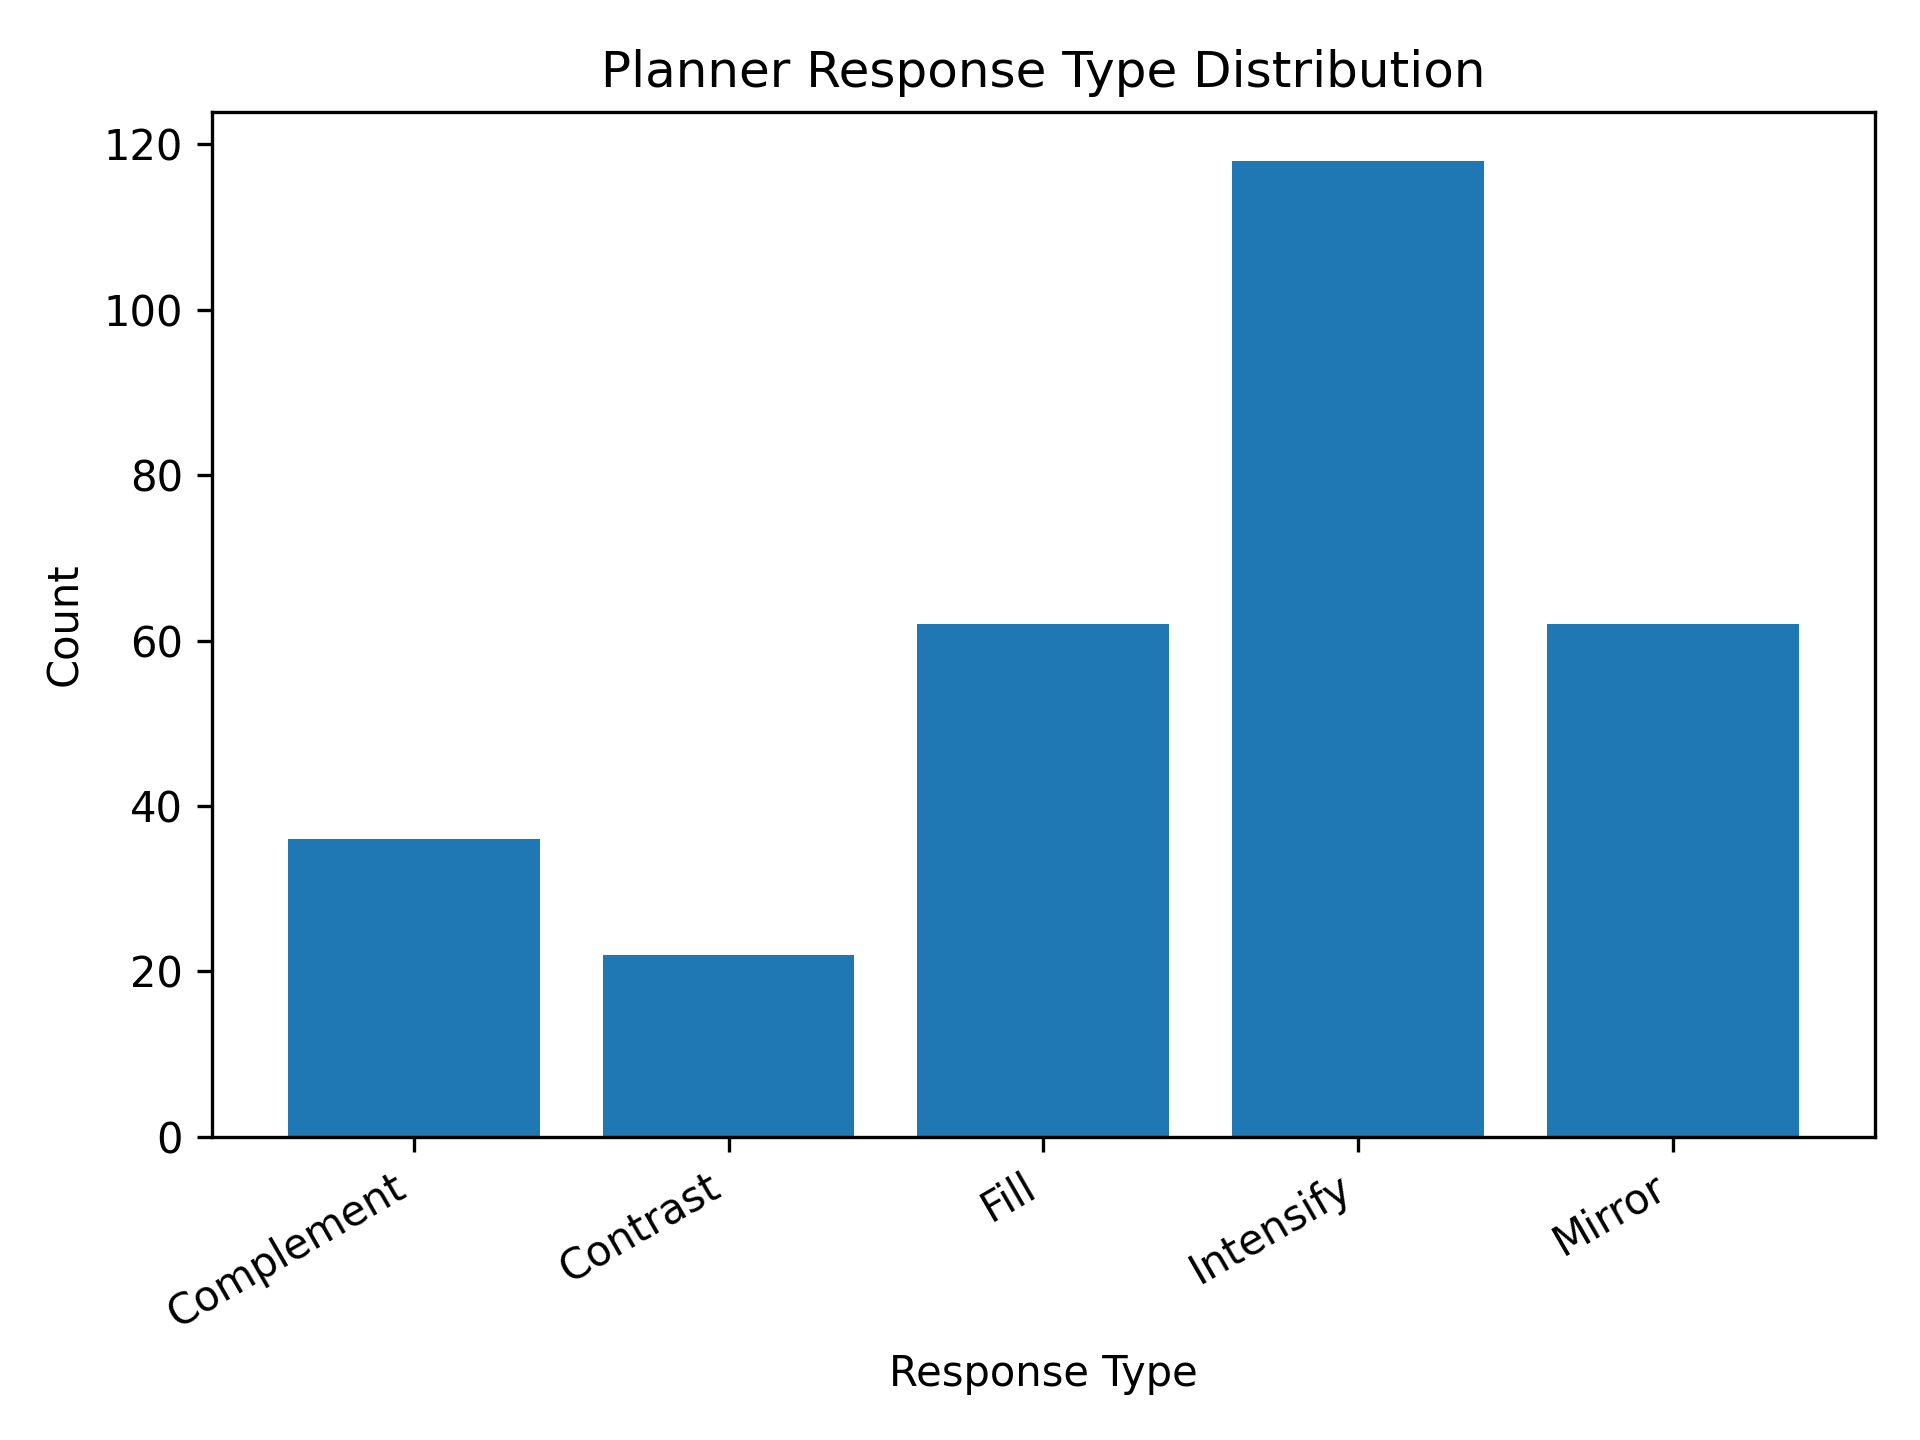
\includegraphics[width=\textwidth]{Figures/5.3 Figs/Figure 5.2 - Planner Response Type Distribution.png}
\caption{Distribution of selected response types across evaluated planner cases.}
\label{fig:planner-response-type-distribution}
\end{figure}

The results indicate that all response types are represented, with
Intensify occurring most frequently (118 cases, 39.3\%), followed by
Fill and Mirror (62 cases each, 20.7\%), Complement (36 cases, 12.0\%)
and Contrast (22 cases, 7.3\%). This confirms that the planner generates
structurally varied responses rather than defaulting to a single
behaviour.

However, the distribution is not uniform. The dominance of Intensify
indicates input patterns within the evaluated dataset more frequently
satisfy the conditions associated with energy or density expansion. This
asymmetry reflects both the planner's scoring structure and the
characteristics of the input set, revealing response selection as being
shaped by underlying feature distributions rather than being arbitrarily
balanced.

\subsection{Decision margins and ambiguity}\label{decision-margins-and-ambiguity}

To assess the robustness of planner decisions, the distribution of
decision margins was analysed (Figure~\ref{fig:planner-decision-margin-distribution}). Decision confidence is
represented by a margin indicating the difference between the
highest-scoring response type and its nearest competitor.

\begin{figure}[htbp]
\centering
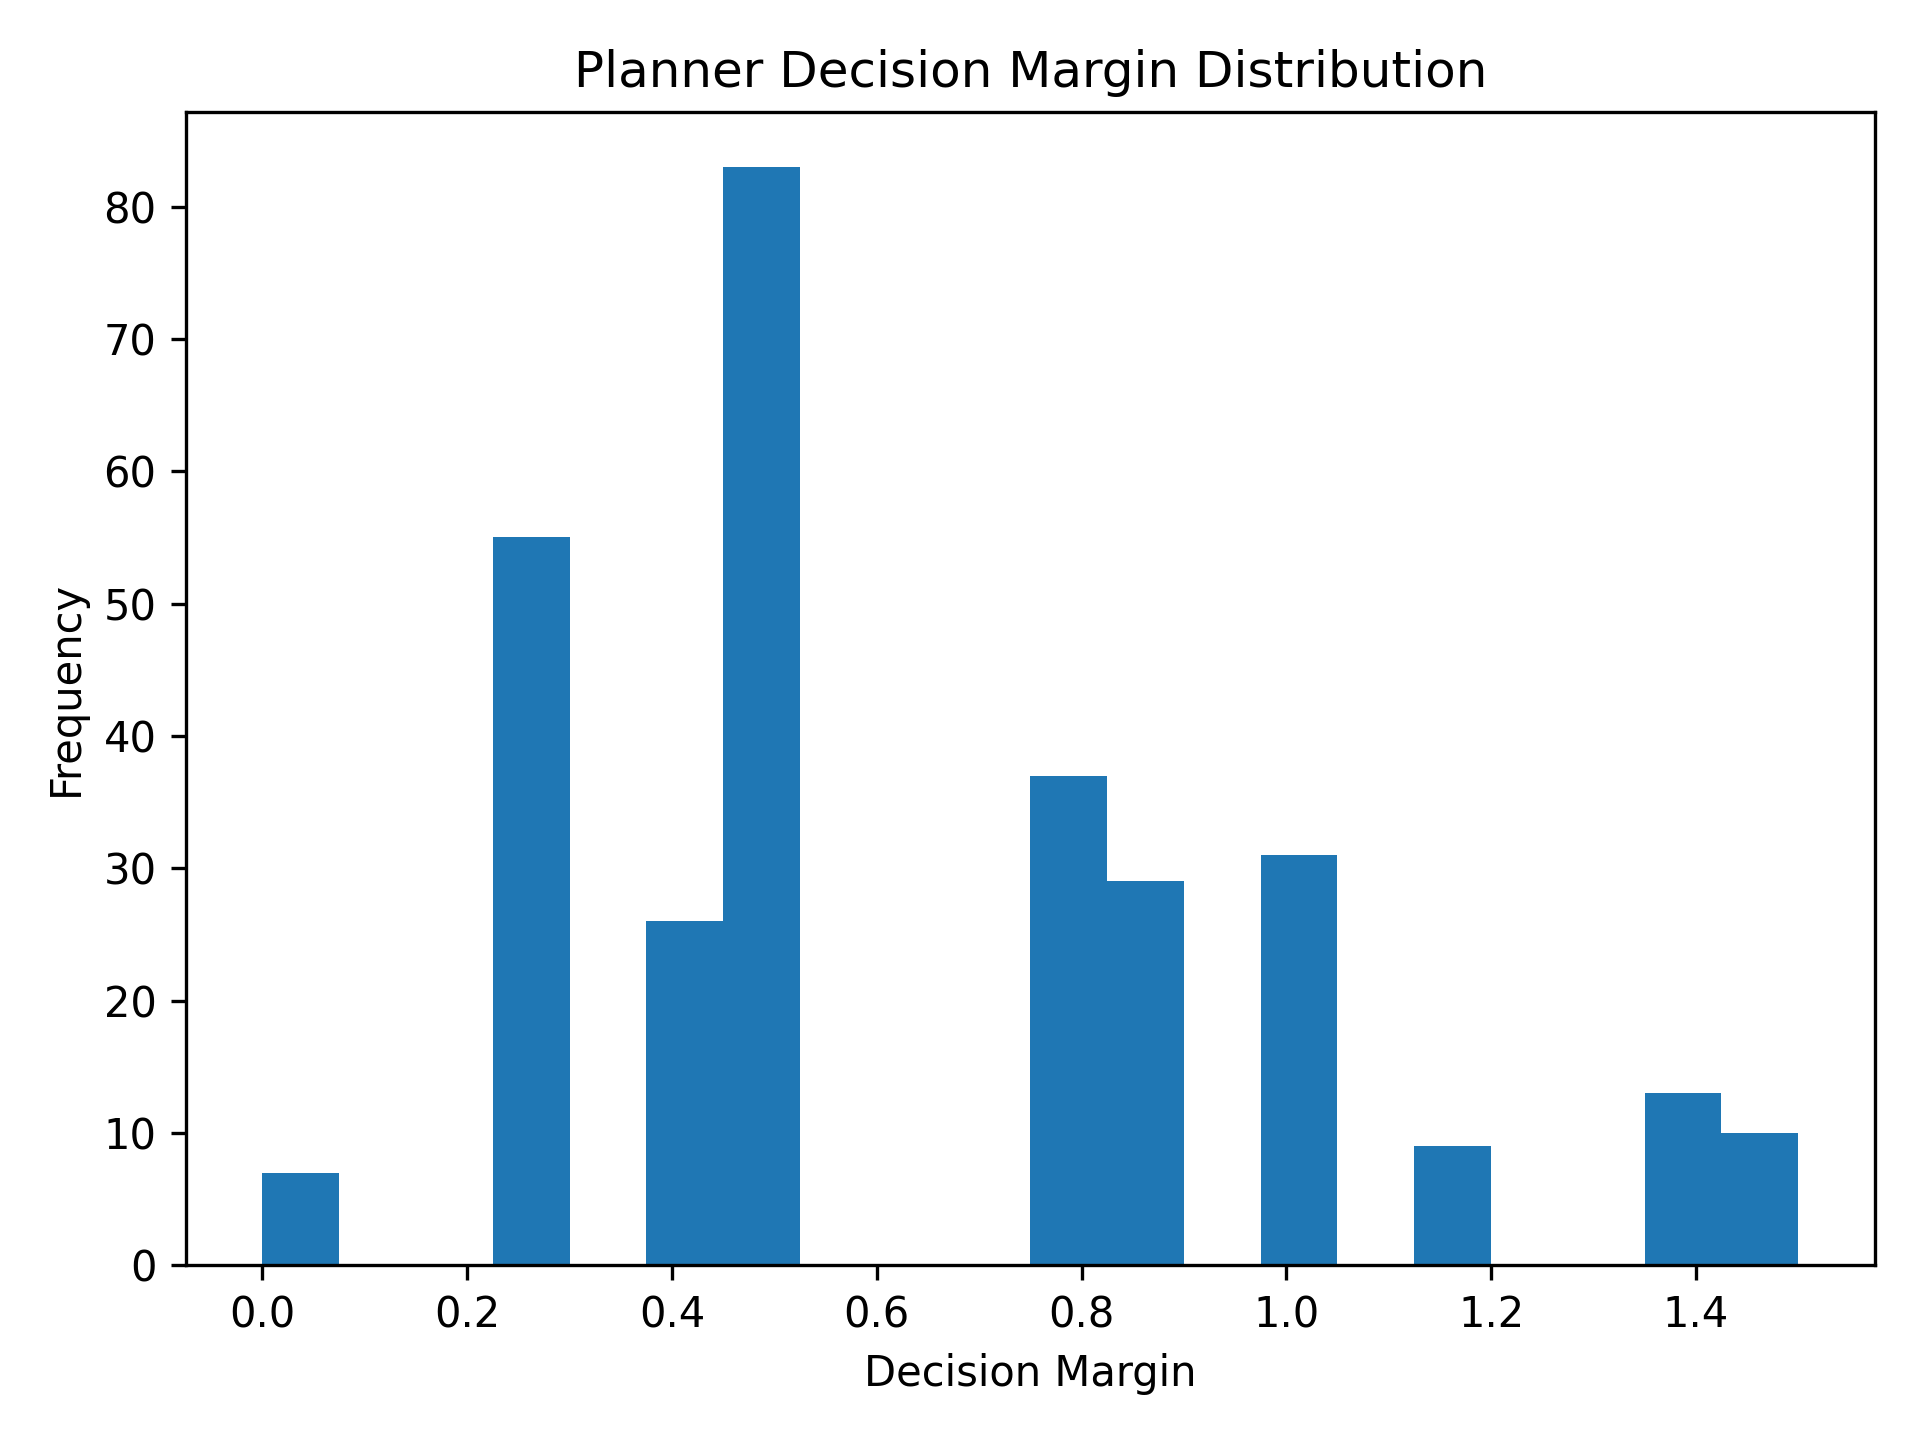
\includegraphics[width=\textwidth]{Figures/5.3 Figs/Figure 5.3 - Planner Decision Margin Distribution.png}
\caption{Distribution of planner decision margins across evaluated cases.}
\label{fig:planner-decision-margin-distribution}
\end{figure}

The results show a wide spread of margins, ranging from near-zero to
approximately 1.5. High-margin cases correspond to strong, unambiguous
decisions, while low-margin cases indicate boundary conditions where
multiple response types are plausible. Importantly, these boundary cases
are explicitly visible rather than hidden, allowing inspection of
competing responses and their associated scores.

This behaviour reflects a key design property of the planner. Rather
than enforcing rigid categorical separation, it operates as a rule-based
system with continuous decision boundaries, where ambiguity is not only
expected and interpretable but potentially musically beneficial because
of the stochasticity it offers. Low-margin cases therefore do not
represent failure, but instead highlight regions of the feature space
where multiple musical interpretations are viable.

\subsection{Interpretability of planner decisions}\label{interpretability-of-planner-decisions}

A central design objective of the system is that response behaviour
should be explainable in terms of explicit rhythmic features. Figure~\ref{fig:planner-decision-trace} presents a representative planner decision trace, illustrating the transformation from input pattern to analysed features, response scores and final selection.

\begin{figure}[htbp]
\centering
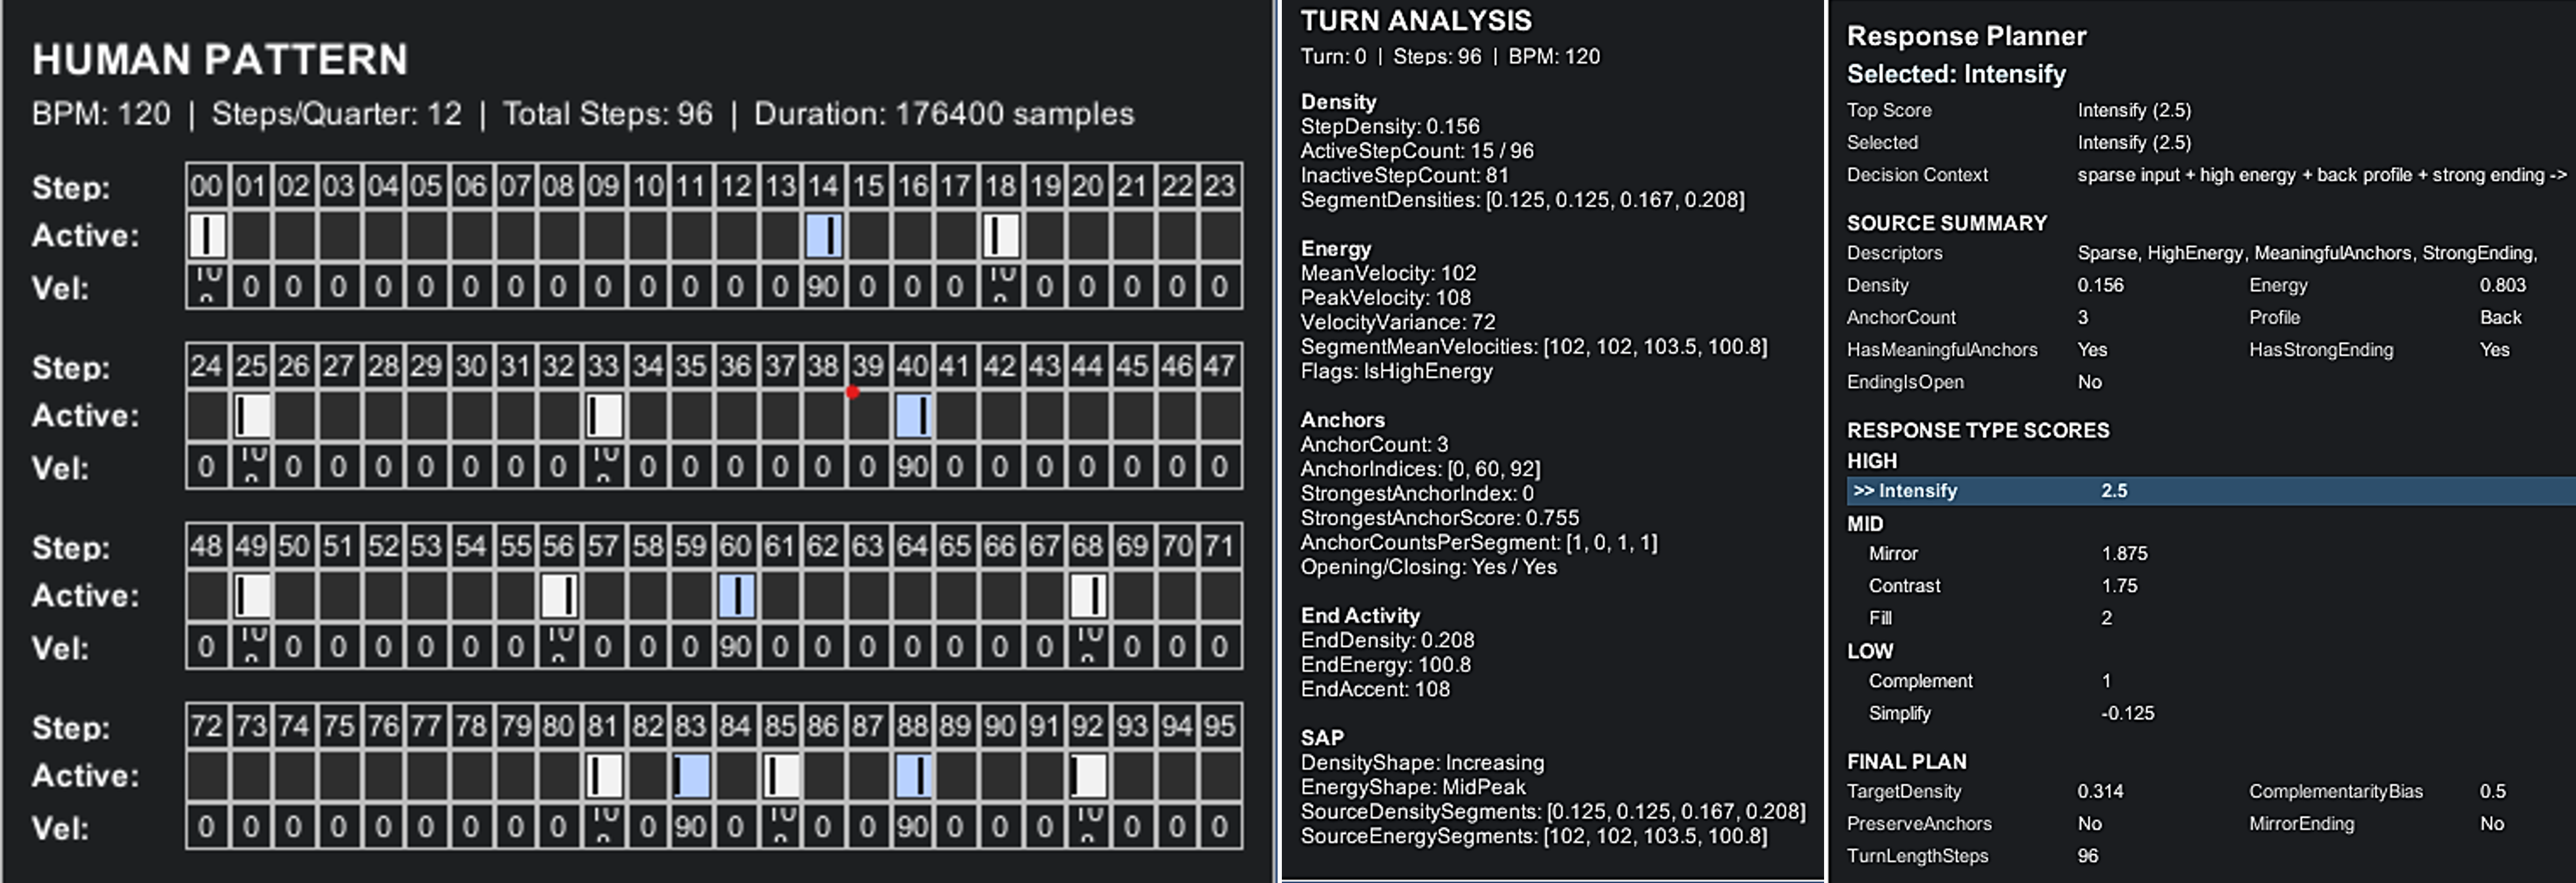
\includegraphics[width=\textwidth]{Figures/5.3 Figs/Figure 5.4 - Planner Decision Trace.png}
\caption{Representative planner decision trace linking input features to response selection.}
\label{fig:planner-decision-trace}
\end{figure}

In this example, a sparse input pattern with high energy, meaningful
anchors and a strong ending leads to the selection of the Intensify
response type. This decision is supported by the planner's scoring
output, where Intensify achieves the highest score (2.5), exceeding
competing response types such as Mirror (1.875), Contrast (1.75) and
Fill (2.0). The associated descriptors - Sparse, HighEnergy,
MeaningfulAnchors, StrongEnding - provide the direct explanation for an
intensification-based response, reflecting the system's tendency to
reinforce energetic and structurally salient input.

Crucially, the decision is not only visible but interpretable at
multiple levels. The selected response can be traced from high-level
descriptors down to underlying feature values, including density, energy
and anchor distribution. Unlike earlier boundary-case examples, this
instance exhibits a clear margin between the top-scoring response and
its competitors, indicating a confident decision rather than an
ambiguous one.

This interpretability is reinforced by the planner's internal
diagnostics, which explicitly compute decision margins and identify
low-confidence cases. Together, these mechanisms ensure that planner
behaviour is not opaque, but instead forms a transparent and inspectable
mapping spanning input features to response intentions. In contrast to
low-margin cases discussed in Section 5.3.2, this example illustrates a
high-confidence decision, demonstrating the planner's ability to
differentiate between ambiguous and strongly defined input conditions.

\subsection{Reactivity to input variation}\label{reactivity-to-input-variation}

Beyond interpretability, the planner must demonstrate reactivity:
changes in input structure should lead to corresponding changes in
response selection. This property is evaluated using variant sensitivity
analysis, where controlled modifications are applied to input patterns.

Figure~\ref{fig:variant-sensitivity} shows the proportion of cases in which the selected response type changes under different input variations. The results indicate that
response changes occur in a substantial proportion of cases across
multiple variant groups, with rates typically ranging between
approximately 10\% and 40\%.

\begin{figure}[htbp]
\centering
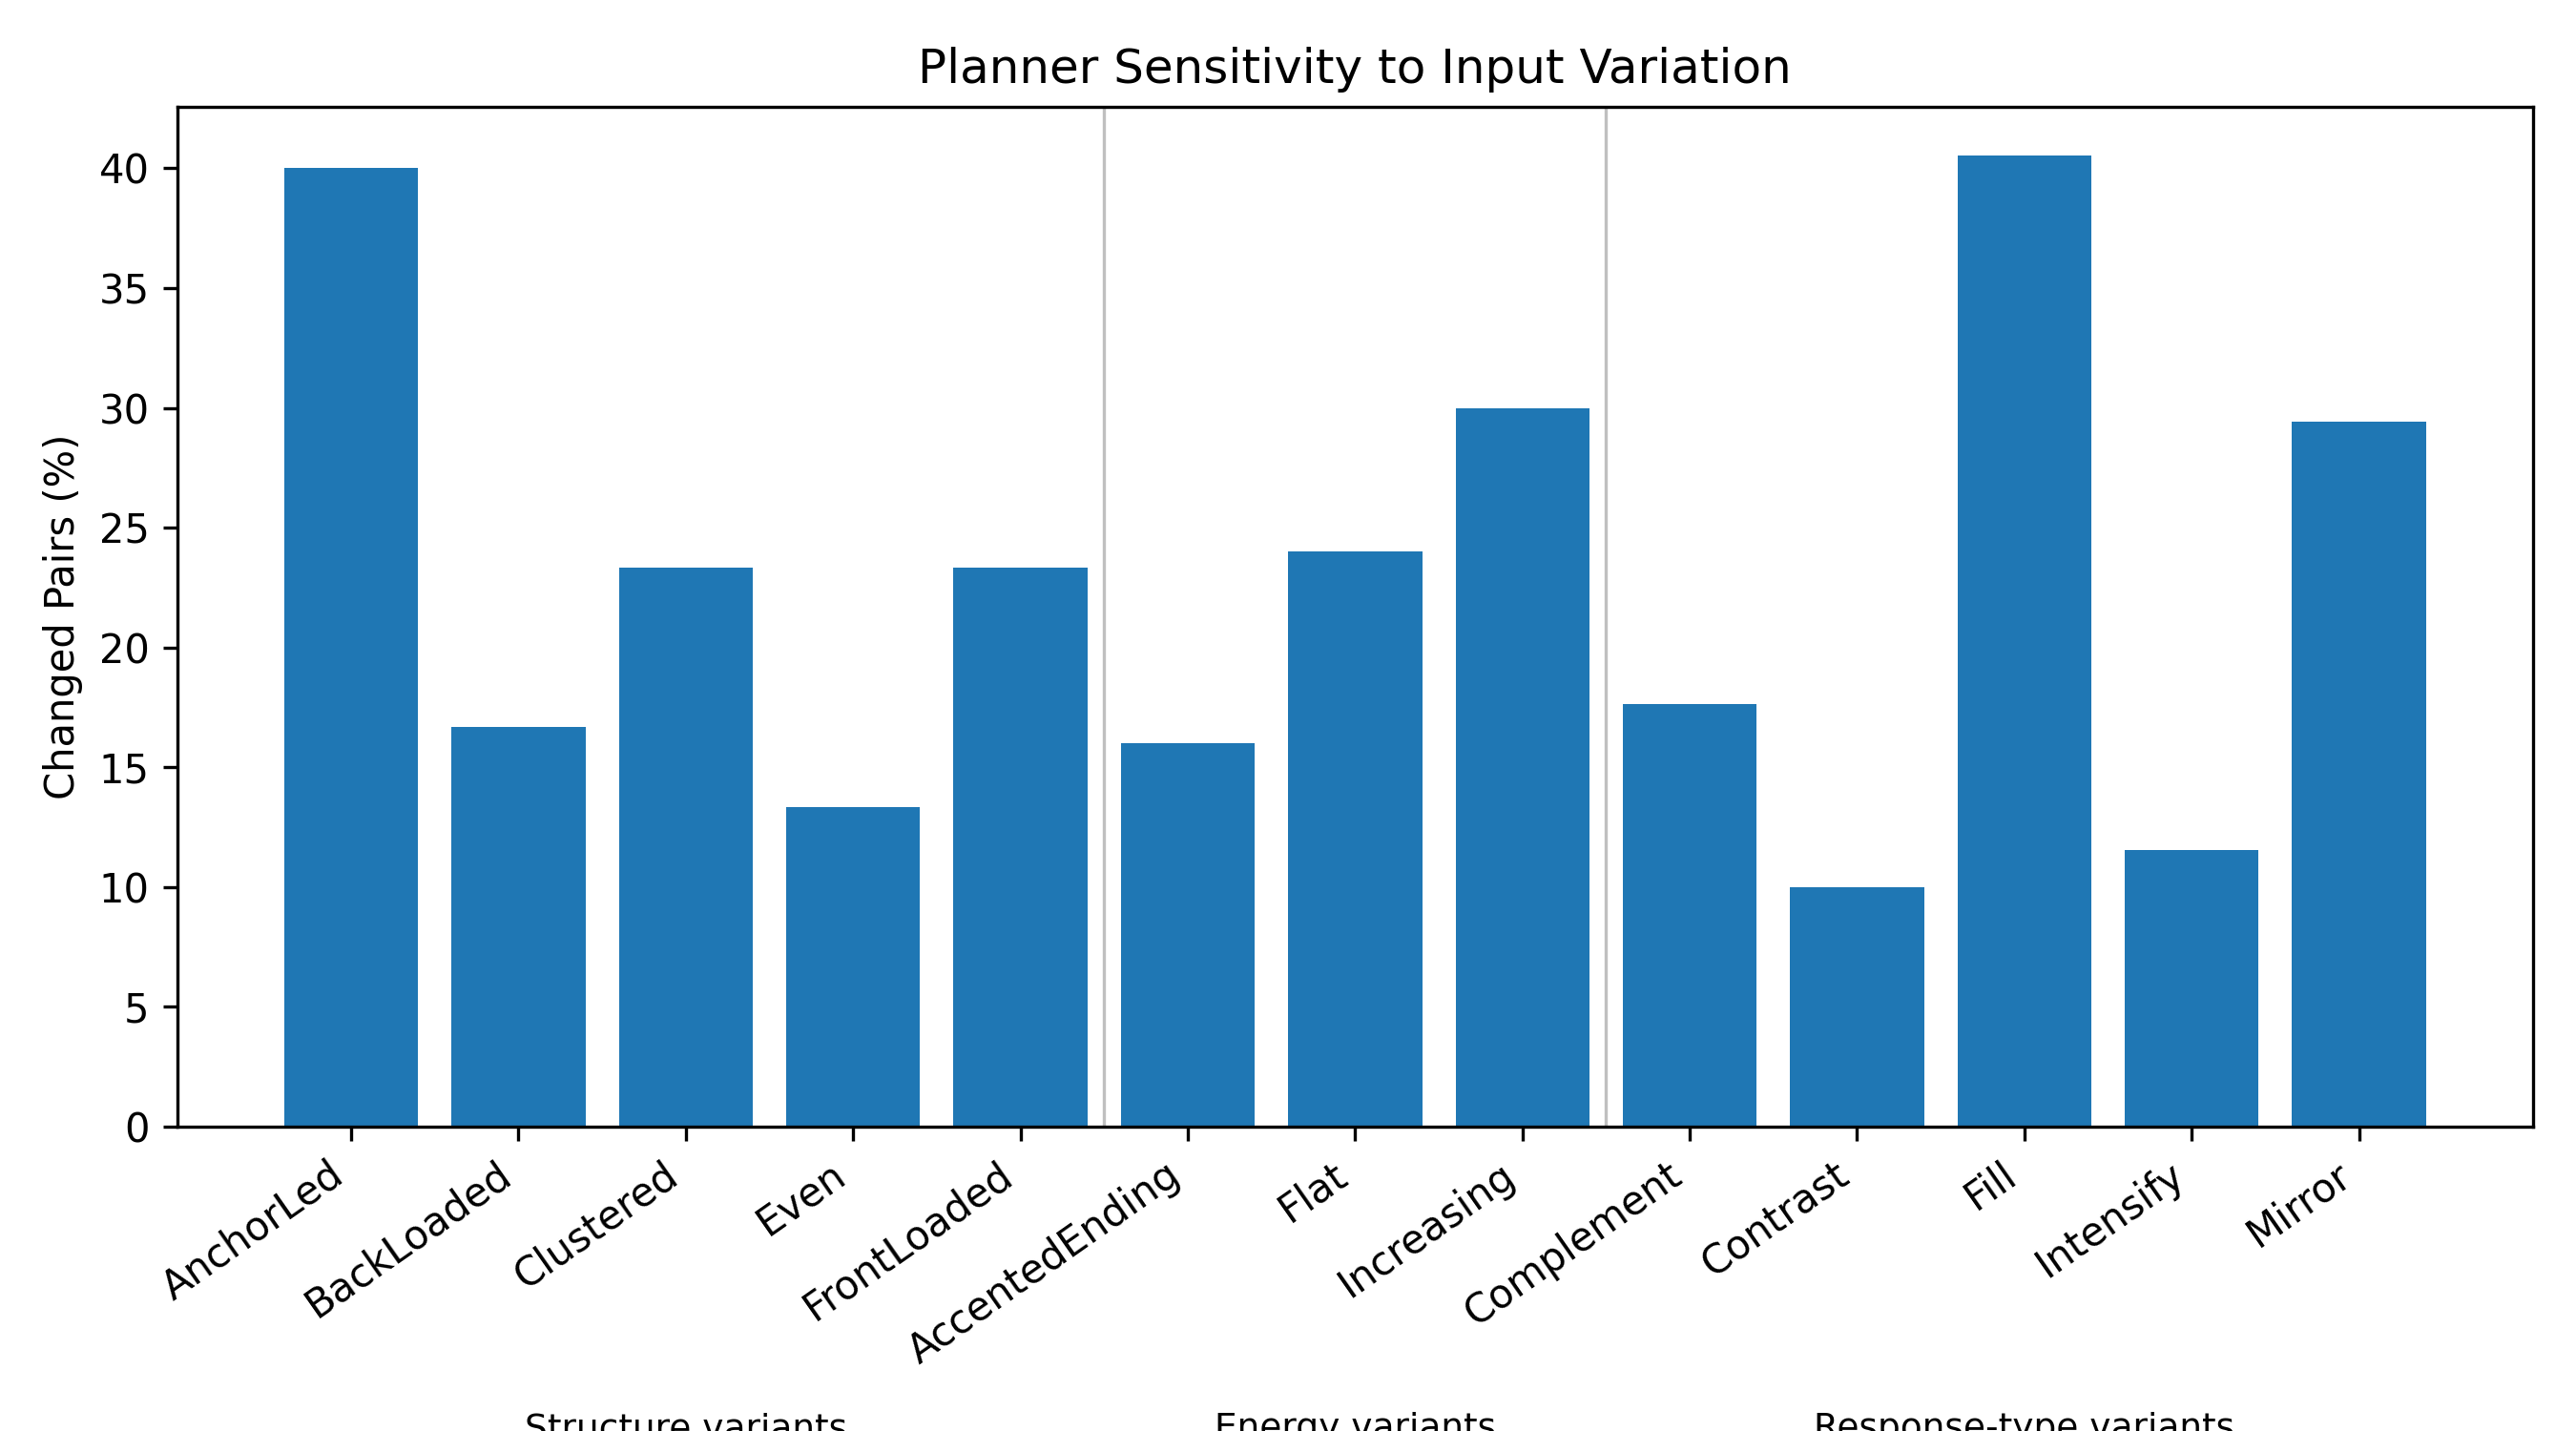
\includegraphics[width=\textwidth]{Figures/5.3 Figs/Figure 5.5 - Variant Sensitivity.png}
\caption{Planner response sensitivity under controlled input variations.}
\label{fig:variant-sensitivity}
\end{figure}

This demonstrates that the planner is not static, but instead responds
meaningfully to variations in structural, energetic and temporal
features. Notably, these changes are not random, they occur in relation
to the specific modifications applied, revealing a tangible relationship
between input characteristics and planner condition.

From an interaction perspective, this is a critical property. Since IT4s
is designed as a turn-based collaborative system, the ability of the
planner to alter its behaviour in response to changes in the human input
is a key indicator of responsiveness. The observed sensitivity therefore
supports the claim that the system operates as a reactive partner rather
than a passive generator.

\subsection{Interim interpretation}\label{interim-interpretation}

These results taken together demonstrate the response planner to be
structured, interpretable and input-sensitive. It yields variable
response types across a diverse set of inputs, exposes its decision
boundaries through measurable margins and allows its outputs to be
traced directly to underlying rhythmic features. At the same time,
heterogeneous response distribution coupled with the presence of
boundary cases indicate that planner behaviour is shaped by both its
internal scoring structure and the characteristics of the input data.
These properties position the planner as a transparent and controllable
decision layer within the overall interaction architecture.

\section{Structural Response Distinctiveness}\label{structural-response-distinctiveness}

While the response planner defines an intended behaviour, it is
necessary to evaluate whether this intention is realised as structurally
differentiated output. In particular, the system must demonstrate that
different response types produce distinct rhythmic patterns, rather than
superficial variations of a shared structure. This section evaluates
structural diversity using quantitative metrics and pairwise
comparisons.

\subsection{Distribution of structural divergence}\label{distribution-of-structural-divergence}

Figure~\ref{fig:structural-divergence-distribution} shows the distribution of pairwise structural divergence across generated responses, computed as a distance measure between skeleton patterns based on step activation.

\begin{figure}[htbp]
\centering
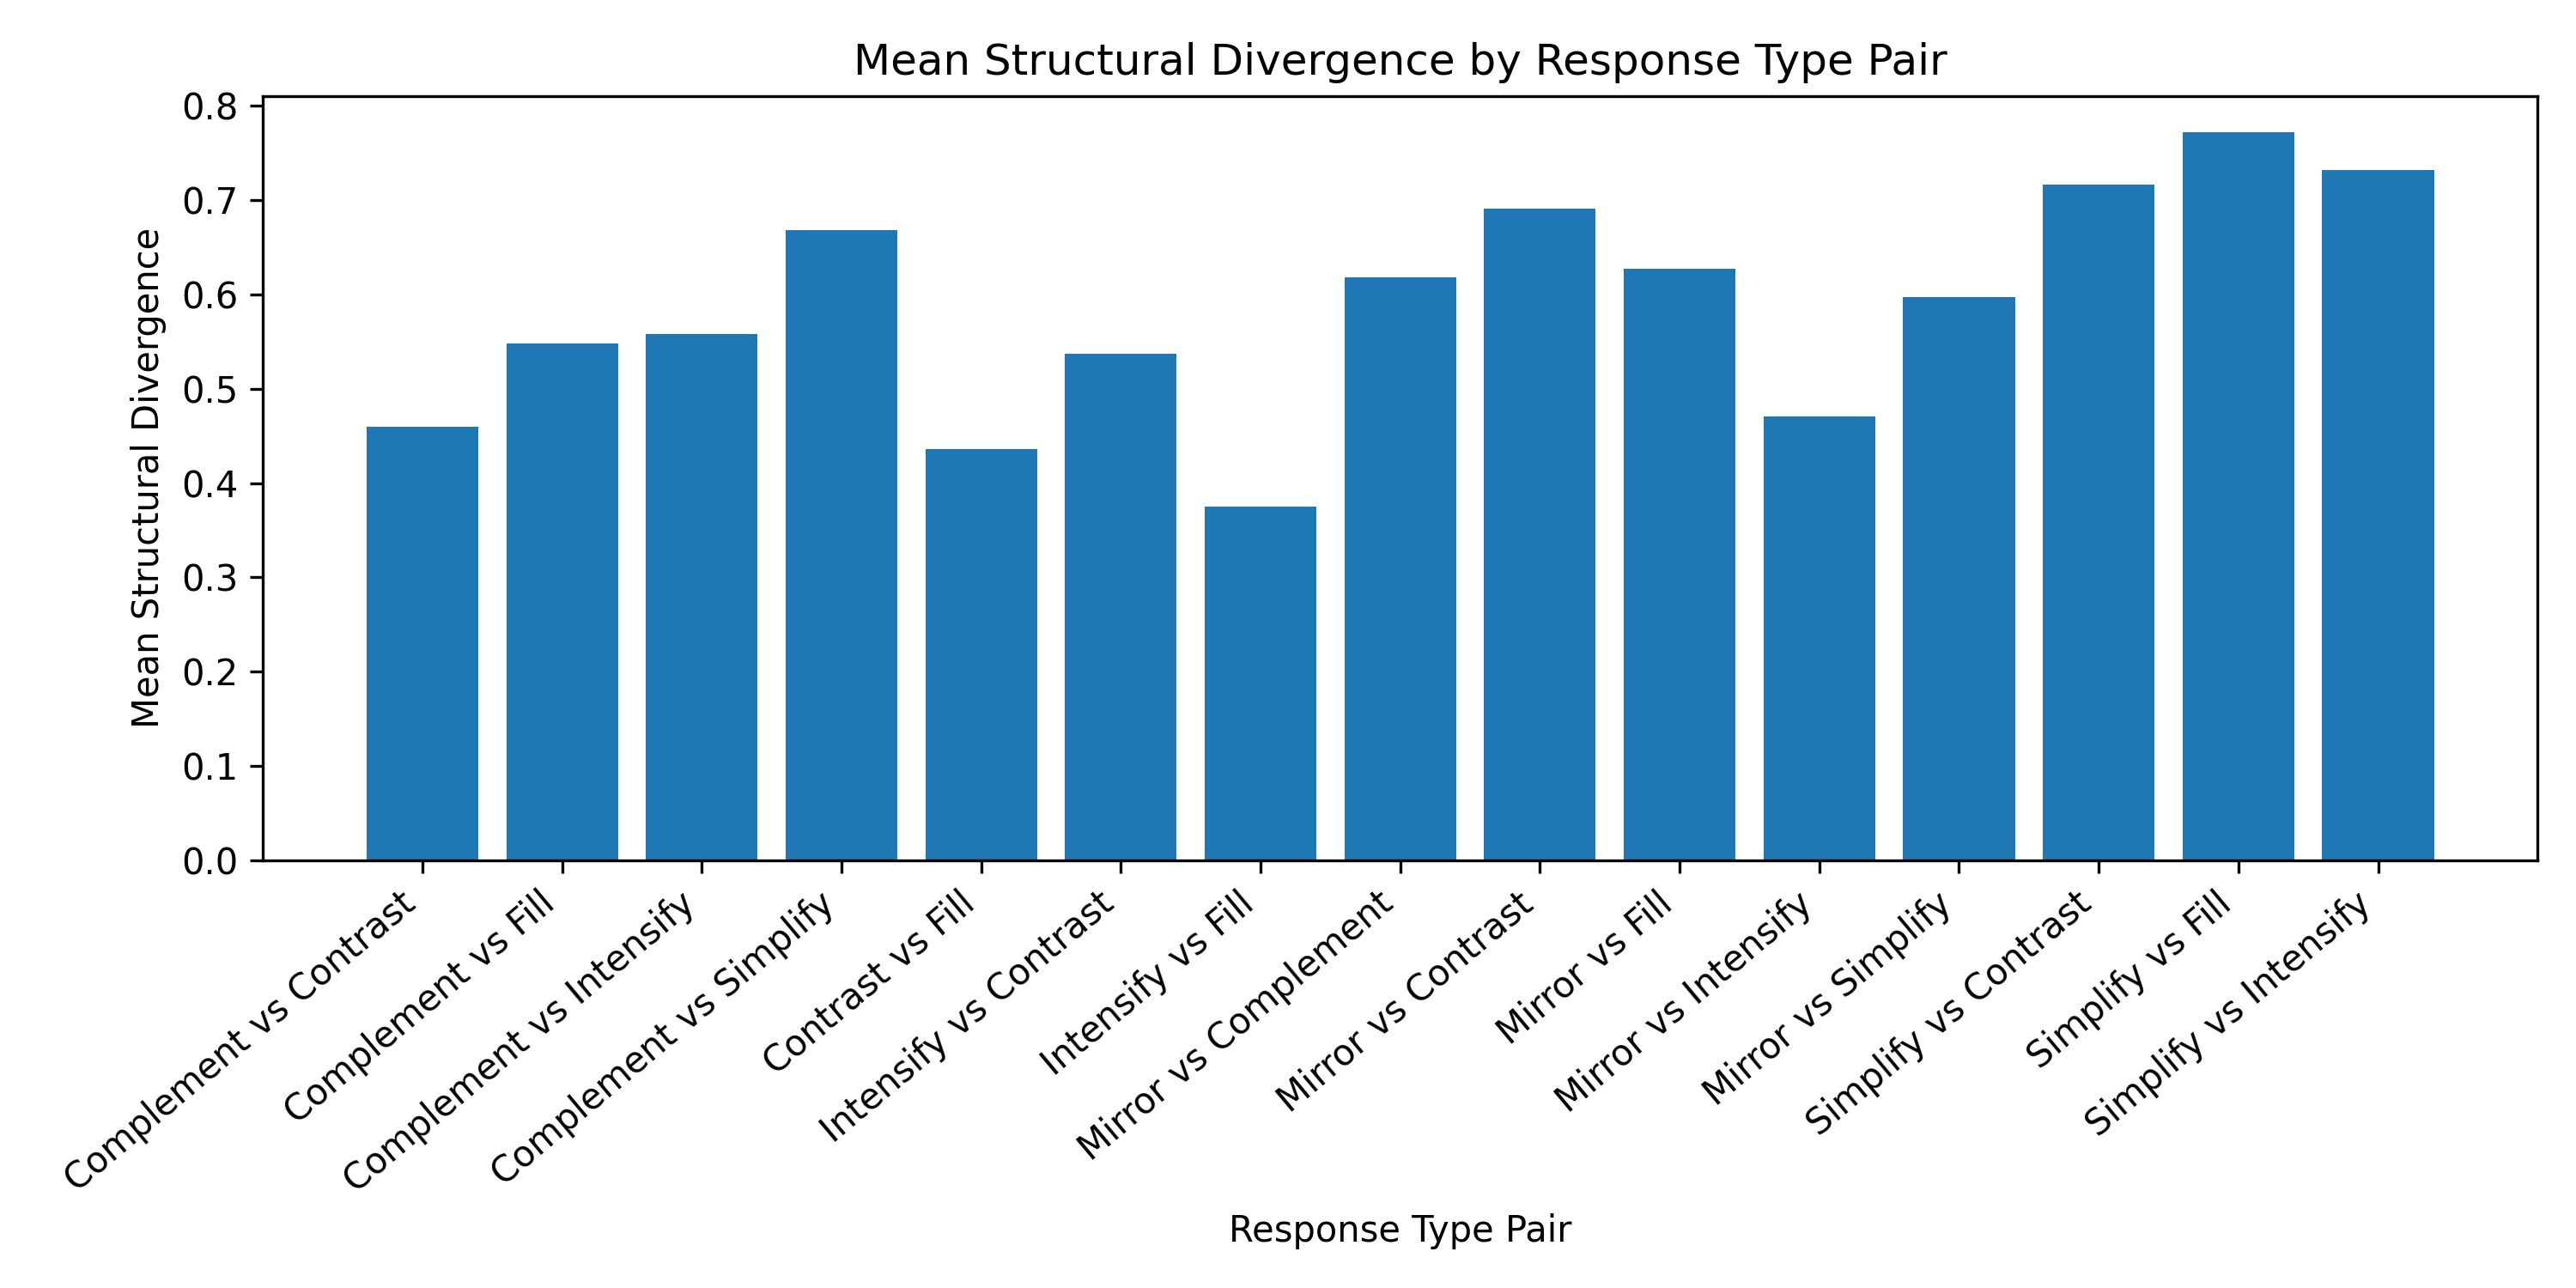
\includegraphics[width=\textwidth]{Figures/5.4 Figs/Figure 5.6 - Structural Divergence Distribution.png}
\caption{Distribution of pairwise structural divergence across generated responses.}
\label{fig:structural-divergence-distribution}
\end{figure}

The distribution exhibits a broad spread, ranging from approximately 0.1
to above 0.9. Crucially, values are not concentrated near zero,
indicating that outputs do not collapse to a single dominant structure.
Instead, the system produces a wide range of structurally distinct
patterns.

This directly supports the claim that the generator avoids structural
degeneracy, producing non-trivial variation across the response space.

\subsection{Structural differences between response types}\label{structural-differences-between-response-types}

While the global divergence distribution demonstrates overall variation,
it does not reveal how response types relate to one another. Figure~\ref{fig:divergence-by-response-type-pair} addresses this by presenting the mean structural divergence between response-type pairs.

\begin{figure}[htbp]
\centering
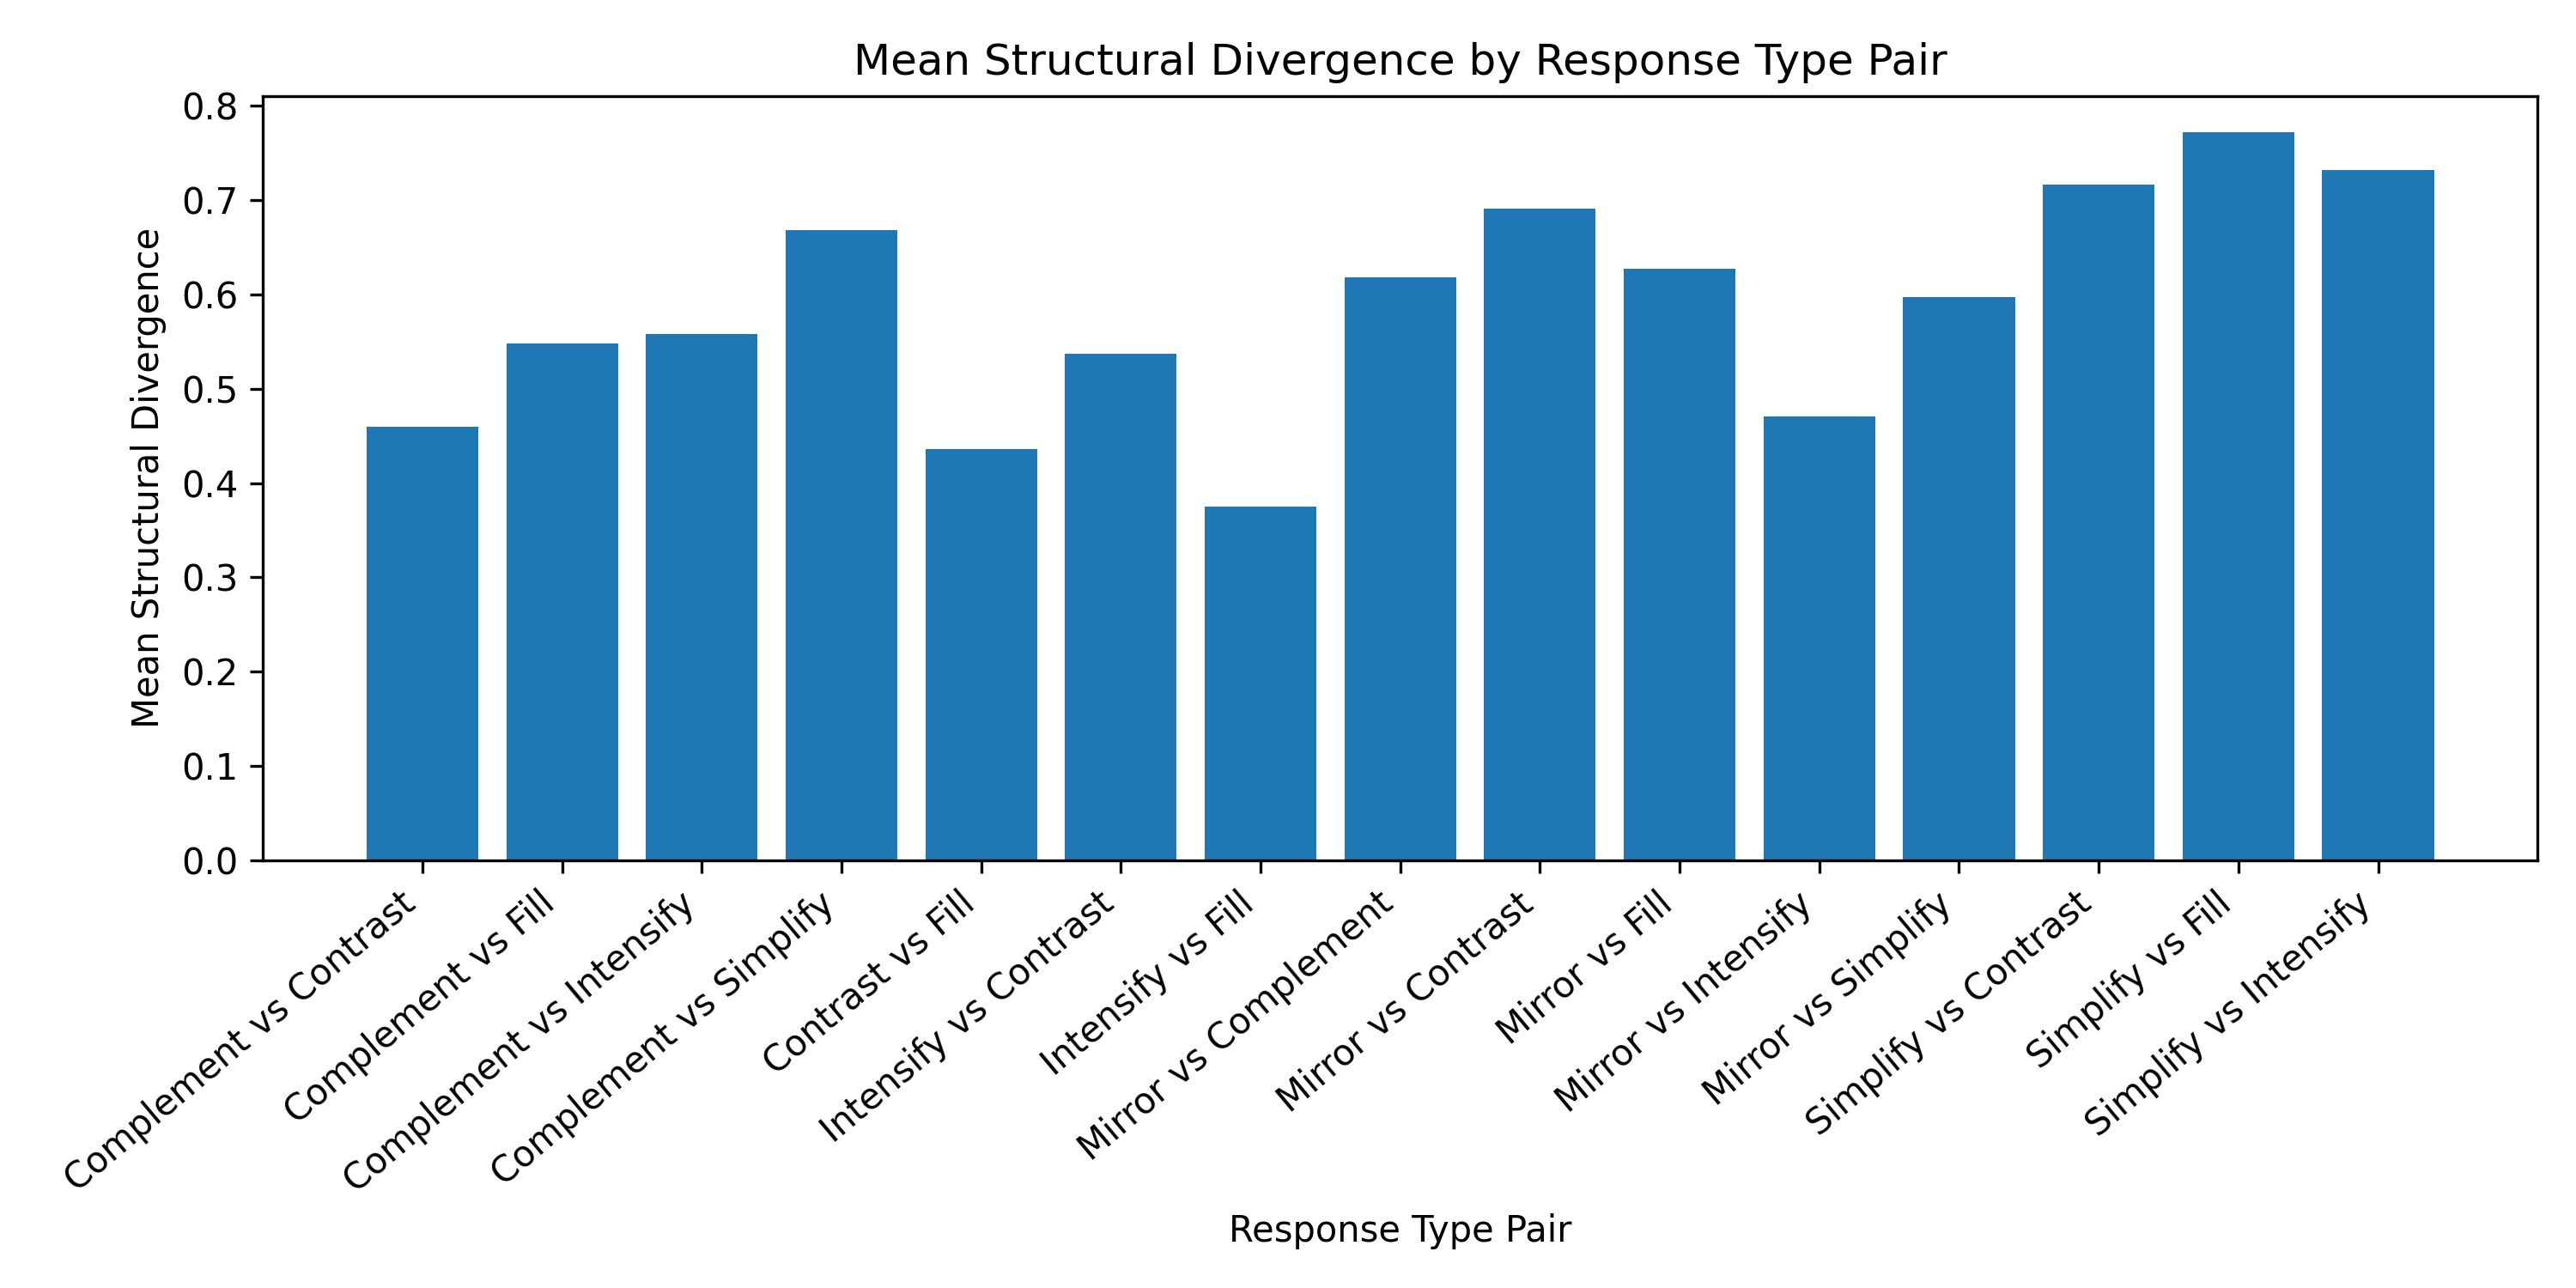
\includegraphics[width=\textwidth]{Figures/5.4 Figs/Figure 5.7 - Divergence by Response-Type Pair.png}
\caption{Mean structural divergence grouped by response-type pair.}
\label{fig:divergence-by-response-type-pair}
\end{figure}

Clear variation is observed across pairs. For example, combinations
involving Simplify (e.g., Simplify vs Fill, Simplify vs Intensify)
exhibit some of the highest divergence values, reflecting strong
differences between sparse and dense behaviours. In contrast, pairs such
as Mirror vs Intensify show comparatively lower divergence, indicating
partial structural similarity despite differing intent.

This demonstrates that variation is not random, but systematically
aligned with response-type semantics. The generator therefore encodes
meaningful behavioural distinctions rather than producing arbitrary
pattern differences.

\subsection{Structural characteristics of response types}\label{structural-characteristics-of-response-types}

Table~\ref{tab:structural-metrics-summary} summarises structural metrics for each response type, including density, number of active steps, anchor preservation, overlap and gap-filling behaviour.

\begin{table}[htbp]
\centering
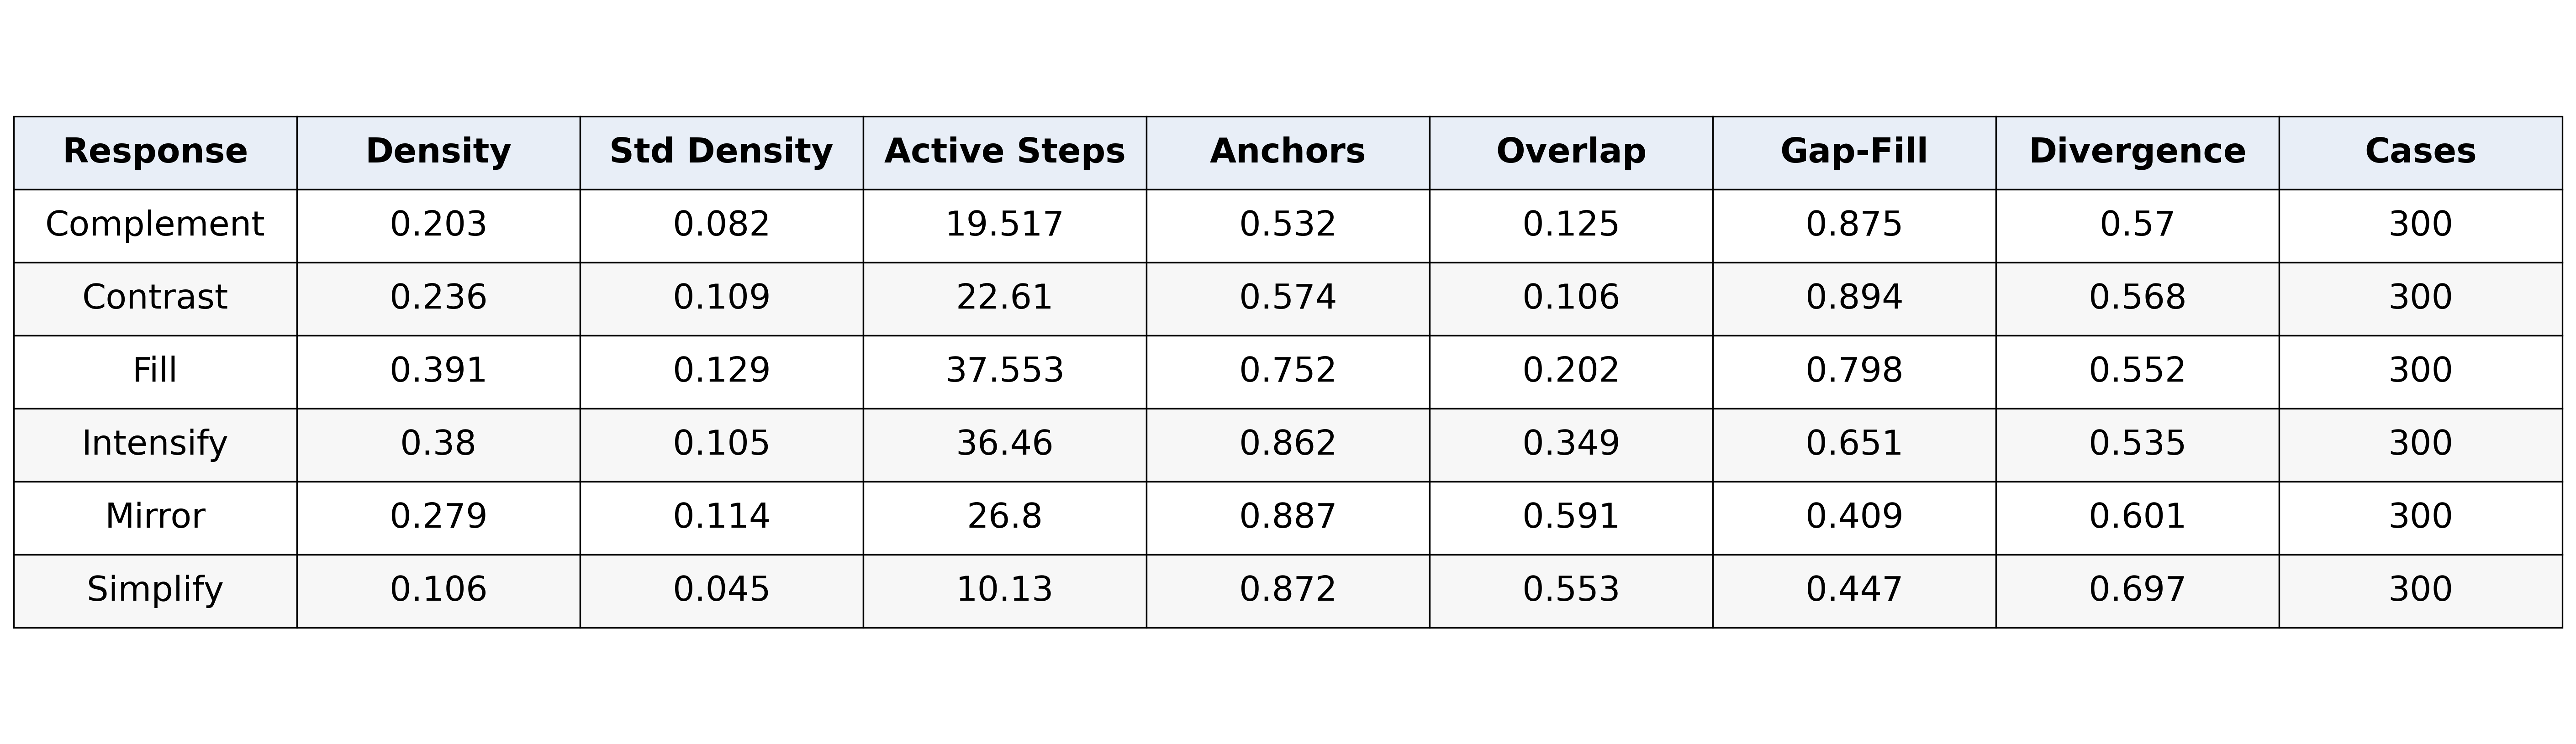
\includegraphics[width=\textwidth]{Figures/5.4 Figs/Table 5.4 - Structural Metrics Summary.png}
\caption{Structural metrics summary by response type.}
\label{tab:structural-metrics-summary}
\end{table}

Clear distinctions emerge:

\begin{itemize}
\item
  Fill and Intensify produce the highest densities (\(\approx\)0.39 and \(\approx\)0.38),
  reflecting expansion of rhythmic activity
\item
  Simplify produces substantially lower density (\(\approx\)0.11), indicating
  strong reduction
\item
  Mirror and Simplify exhibit the highest anchor preservation (\(\approx\)0.89 and
  \(\approx\)0.87)
\item
  Complement and Contrast show higher gap-filling behaviour and reduced
  overlap
\end{itemize}

These differences align with the intended semantics of each response
type, providing evidence that structural properties are not arbitrary,
but reflect the planner's behavioural definitions.

\subsection{Interpretation of structural variation}\label{interpretation-of-structural-variation}

Taken together, the divergence distribution, pairwise comparisons and
summary metrics demonstrate that the system produces structurally
differentiated outputs across response types. Variation is observed both
globally and systematically.

However, structural distinctiveness alone is insufficient to demonstrate
successful response generation, as it does not guarantee alignment with
planned behaviour. A pattern may be structurally distinct while still
deviating from intended parameters such as density or anchor usage.

Structural variation should therefore be interpreted as a necessary but
not sufficient condition for correct response realisation.

\subsection{Interim interpretation}\label{interim-interpretation-1}

This section demonstrates that Intelli-Trading Fours produces diverse
and systematically differentiated rhythmic outputs. The generator avoids
structural collapse and encodes distinct response-type behaviours.
However, structural variation alone does not ensure fidelity to planner
intent, motivating further analysis of plan-to-output alignment in the
following section.

\section{Plan-to-Output Fidelity and Limitations}\label{plan-to-output-fidelity-and-limitations}

While Section 5.3 demonstrated that the planner produces interpretable
decisions and Section 5.4 established that outputs are structurally
distinct, it remains necessary to evaluate how accurately these outputs
reflect the planner's intended behaviour. This section examines
plan-to-output fidelity, focusing on the extent to which planned
parameters are realised during generation.

\subsection{Density as a proxy for fidelity}\label{density-as-a-proxy-for-fidelity}

To quantify fidelity, the difference between the planner's target
density and the realised output density was measured. Figure~\ref{fig:plan-output-density-error} shows the mean density error across response types.

\begin{figure}[htbp]
\centering
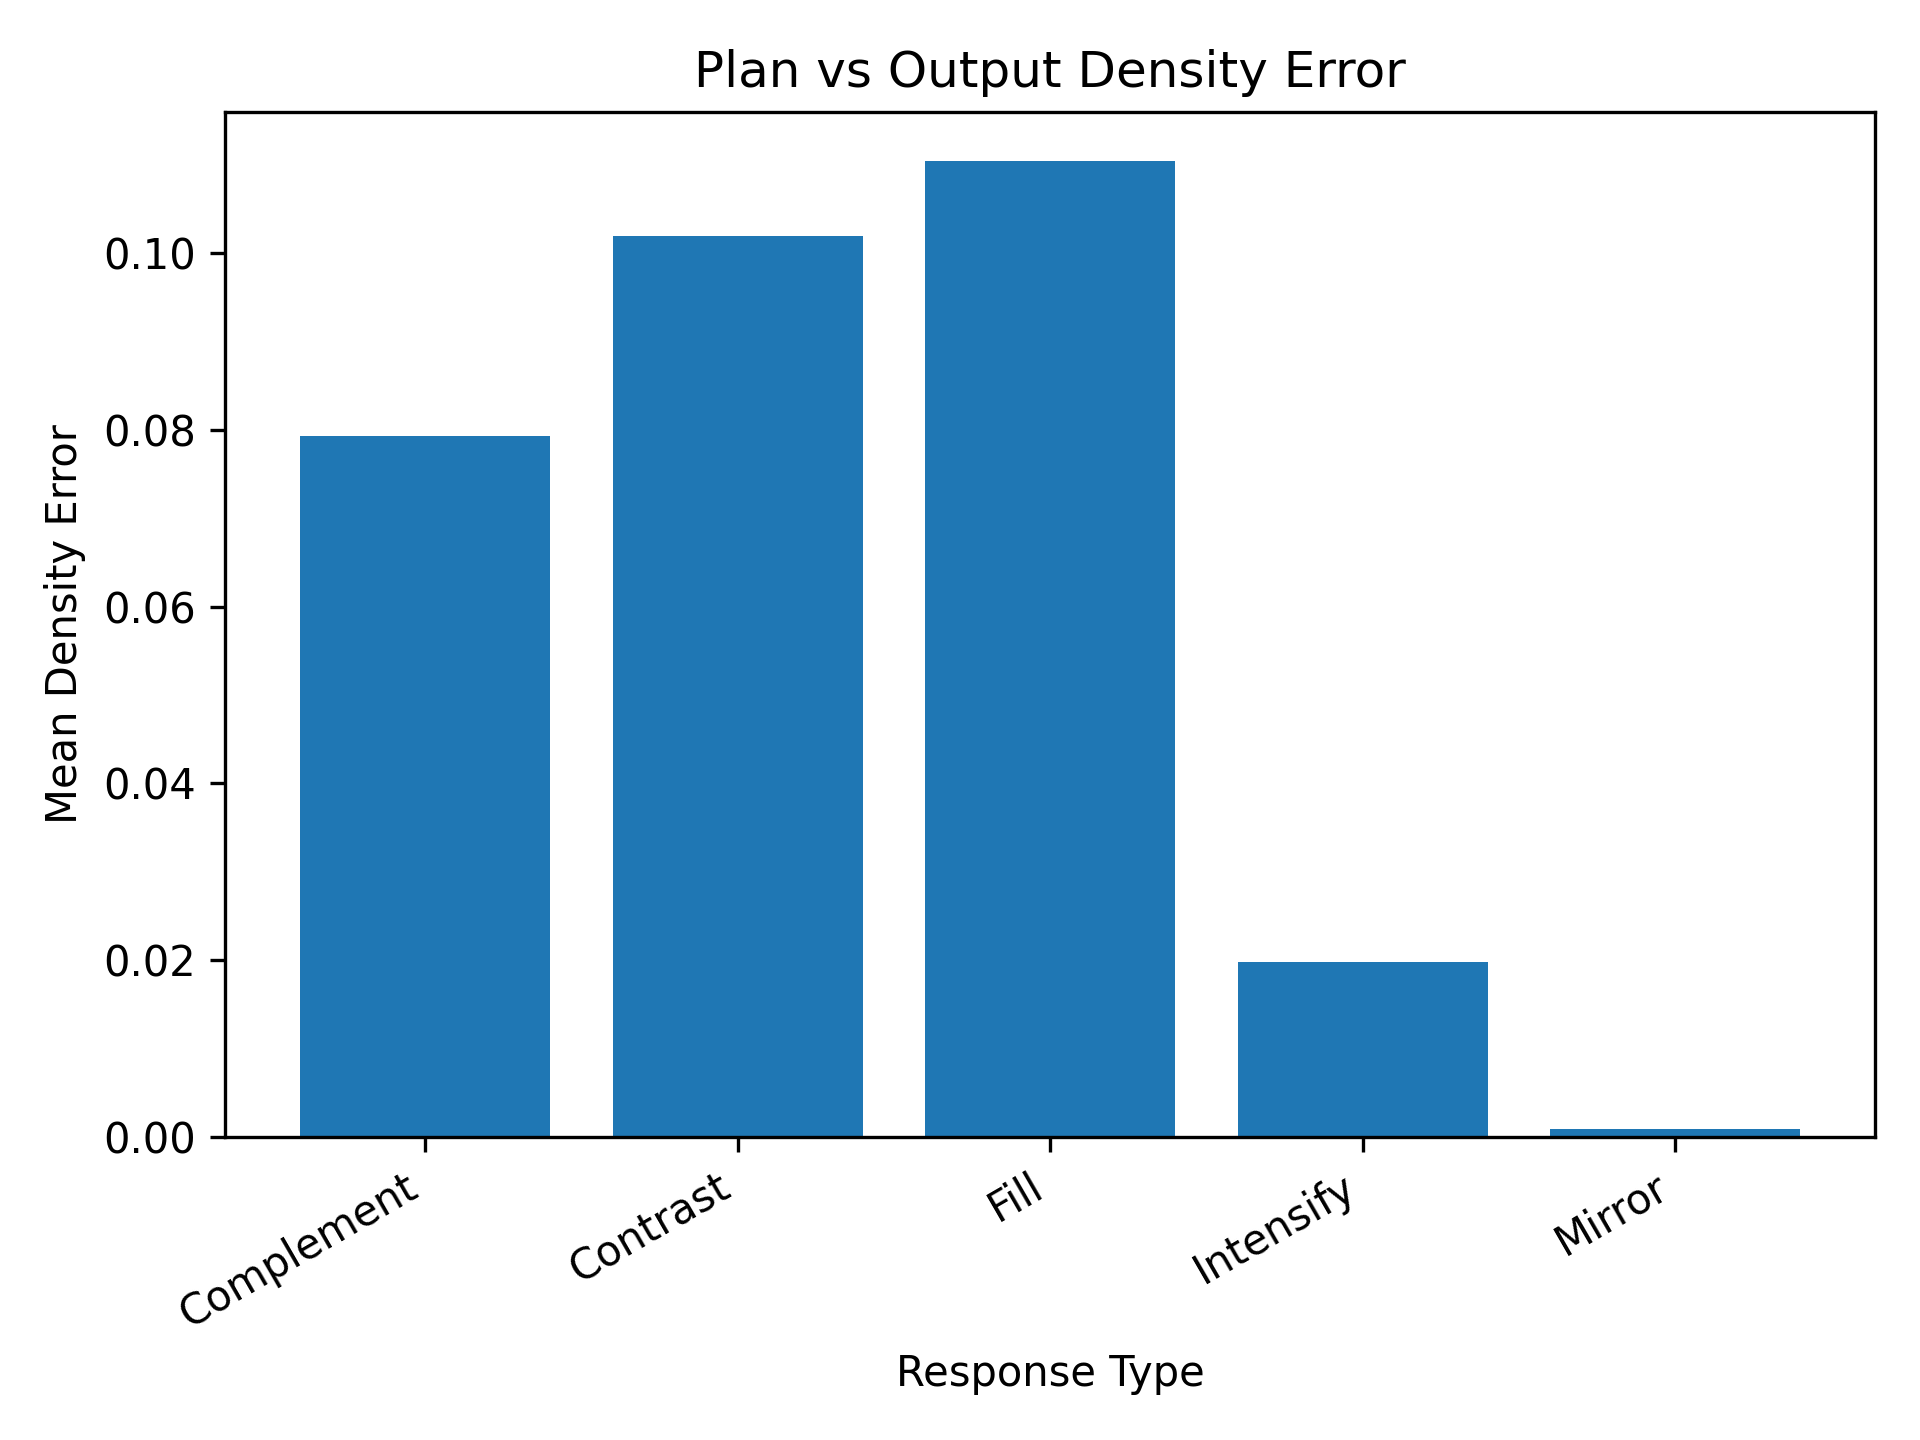
\includegraphics[width=\textwidth]{Figures/5.5 FIgs/Figure 5.6 Plan vs Output Density Eroror.png}
\caption{Mean plan-to-output density error by response type.}
\label{fig:plan-output-density-error}
\end{figure}

This provides a direct quantitative measure of divergence between
planner intent and realised output, operationalising the architectural
separation identified in Section 4.6.

The results indicate significant variation in fidelity:

\begin{itemize}
\item
  Mirror exhibits near-zero error, indicating accurate reproduction of
  source structure
\item
  Intensify shows relatively low error, suggesting effective
  amplification of activity
\item
  Complement, Contrast and particularly Fill exhibit higher error
\end{itemize}

These response types require more complex structural transformations,
including redistribution of activity and deviation from existing
anchors. The increased error indicates reduced fidelity in these cases.

\subsection{Interpretation of fidelity differences}\label{interpretation-of-fidelity-differences}

A clear asymmetry emerges: response types involving preservation or
reinforcement of existing structure (e.g., Mirror, Intensify) are
realised more accurately than those requiring structural
reinterpretation (e.g., Complement, Contrast, Fill).

This reflects a bias in the current generation mechanism toward
structure-preserving transformations. The SkeletonBuilder operates
through constrained step selection, prioritising metric salience,
spacing and anchor-related behaviour. While effective for reinforcement,
this approach provides limited control over more abstract
transformations.

As a result, the generator produces approximations that satisfy local
constraints while only partially fulfilling global planning targets.

\subsection{Implications for system design}\label{implications-for-system-design}

These results clarify the boundary between planning and generation
within the current architecture. The planner successfully produces
differentiated and interpretable intentions, but the generator does not
yet provide a fully expressive mechanism for enforcing those intentions.

This suggests two directions for improvement:

\begin{itemize}
\item
  tighter coupling between planning parameters and generation
  constraints
\item
  more expressive generation mechanisms (e.g., stochastic or learned
  approaches)
\end{itemize}

Such extensions would allow more accurate realisation of
transformation-heavy response types.

\subsection{Interim interpretation}\label{interim-interpretation-2}

This section demonstrates that while Intelli-Trading Fours produces
diverse and interpretable outputs, the realisation of planned behaviour
is not uniform across response types. Fidelity is highest for
structure-preserving behaviours and lowest for transformation-heavy
responses, highlighting a limitation in the current generation approach.

This identifies a key design trade-off between interpretability and
generative fidelity and establishes a clear direction for future
development.

% TODO: Missing latency plot figure source referenced in the evaluation framework.
% TODO: Missing plan-vs-output case table source referenced in the evaluation framework.
% TODO: Add annotated case figures if they become available.
